\documentclass[tikz, border=4pt]{standalone}
% Shared preamble for the qpo_*.tex query plan figures.
\usepackage[T1]{fontenc}
\usepackage{lmodern}
\usetikzlibrary{arrows.meta, positioning, fit, backgrounds, calc}

\definecolor{accent}{HTML}{2F5D8C}
\definecolor{groupfill}{HTML}{EEF3F8}
\definecolor{taskfill}{HTML}{FFFFFF}
\definecolor{note}{HTML}{555555}
\definecolor{hot}{HTML}{C0561B}
\definecolor{hotfill}{HTML}{FCEBDD}

\newcommand{\sub}{\tiny\color{note}}
\newcommand{\hsub}{\tiny\color{hot}}

\tikzset{
    every picture/.style={font=\sffamily\scriptsize, node distance=4mm},
    op/.style={draw=accent, fill=taskfill, rounded corners=2pt, line width=0.6pt,
               minimum width=30mm, minimum height=7mm, align=center, inner sep=2pt},
    tbl/.style={op, fill=groupfill},
    small/.style={minimum width=18mm},
    hot/.style={draw=hot, fill=hotfill, line width=1pt},
    flow/.style={-{Stealth[length=2mm]}, accent, line width=0.7pt},
    hotflow/.style={flow, color=hot, line width=0.9pt},
    panel/.style={draw=accent, dashed, rounded corners=4pt, line width=0.6pt, inner sep=3mm},
    lbl/.style={font=\sffamily\scriptsize\bfseries, text=accent},
    callout/.style={font=\sffamily\tiny, text=hot, align=left},
}

\begin{document}
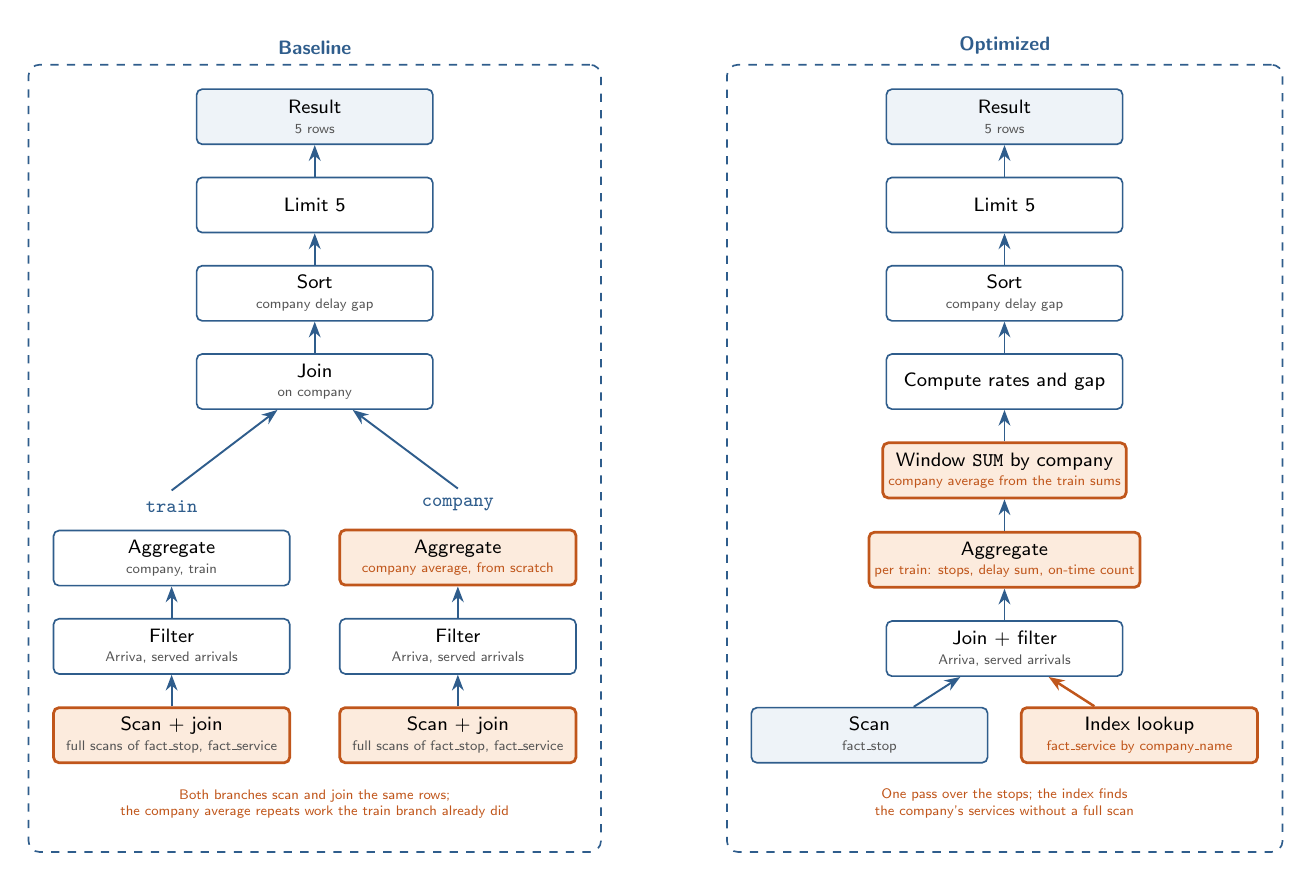
\begin{tikzpicture}

% ---------------- Baseline: two branches ----------------
\node[tbl, hot] (bs1) {Scan + join\\[-1pt]{\sub full scans of fact\_stop, fact\_service}};
\node[op, above=of bs1] (bf1) {Filter\\[-1pt]{\sub Arriva, served arrivals}};
\node[op, above=of bf1] (ba1) {Aggregate\\[-1pt]{\sub company, train}};
\node[lbl, above=1mm of ba1] (bc1) {\texttt{train}};

\node[tbl, hot, right=6mm of bs1] (bs2) {Scan + join\\[-1pt]{\sub full scans of fact\_stop, fact\_service}};
\node[op, above=of bs2] (bf2) {Filter\\[-1pt]{\sub Arriva, served arrivals}};
\node[op, hot, above=of bf2] (ba2) {Aggregate\\[-1pt]{\hsub company average, from scratch}};
\node[lbl, above=1mm of ba2] (bc2) {\texttt{company}};

\draw[flow] (bs1) -- (bf1);
\draw[flow] (bf1) -- (ba1);
\draw[flow] (bs2) -- (bf2);
\draw[flow] (bf2) -- (ba2);

\node[callout, below=2mm of $(bs1.south)!0.5!(bs2.south)$, align=center] (bnote)
    {Both branches scan and join the same rows;\\the company average repeats work the train branch already did};

% ---------------- Optimized ----------------
\node[tbl, right=22mm of bs2] (ost) {Scan\\[-1pt]{\sub fact\_stop}};
\node[tbl, hot, right=4mm of ost] (osv) {Index lookup\\[-1pt]{\hsub fact\_service by company\_name}};
\coordinate (omid) at ($(ost)!0.5!(osv)$);
\node[op] (oj) at ($(omid) + (0, 11mm)$) {Join + filter\\[-1pt]{\sub Arriva, served arrivals}};
\node[op, hot, above=of oj] (oa) {Aggregate\\[-1pt]{\hsub per train: stops, delay sum, on-time count}};
\node[op, hot, above=of oa] (ow) {Window \texttt{SUM} by company\\[-1pt]{\hsub company average from the train sums}};
\node[op, above=of ow] (oc) {Compute rates and gap};
\node[op, above=of oc] (oo) {Sort\\[-1pt]{\sub company delay gap}};
\node[op, above=of oo] (ol) {Limit 5};
\node[op, fill=groupfill, above=of ol] (or) {Result\\[-1pt]{\sub 5 rows}};

\draw[flow] (ost) -- (oj);
\draw[hotflow] (osv) -- (oj);
\draw[flow] (oj) -- (oa);
\draw[flow] (oa) -- (ow);
\draw[flow] (ow) -- (oc);
\draw[flow] (oc) -- (oo);
\draw[flow] (oo) -- (ol);
\draw[flow] (ol) -- (or);

\node[callout, below=2mm of omid |- ost.south, align=center] (onote)
    {One pass over the stops; the index finds\\the company's services without a full scan};

\begin{scope}[on background layer]
  \node[panel, fit=(ost)(osv)(or)(onote)(bnote.south -| ost)] (opp) {};
\end{scope}
\node[lbl, anchor=south] at (opp.north) {Optimized};

% ---------------- Baseline top, aligned with the optimized side ----------------
\coordinate (bmid) at ($(ba1)!0.5!(ba2)$);
\node[op] (bj) at (bmid |- oc) {Join\\[-1pt]{\sub on company}};
\node[op, above=of bj] (bo) {Sort\\[-1pt]{\sub company delay gap}};
\node[op, above=of bo] (bl) {Limit 5};
\node[op, fill=groupfill, above=of bl] (br) {Result\\[-1pt]{\sub 5 rows}};

\draw[flow] (bc1.north) -- (bj);
\draw[flow] (bc2.north) -- (bj);
\draw[flow] (bj) -- (bo);
\draw[flow] (bo) -- (bl);
\draw[flow] (bl) -- (br);

\begin{scope}[on background layer]
  \node[panel, fit=(bs1)(bs2)(br)(bnote)] (bp) {};
\end{scope}
\node[lbl, anchor=south] at (bp.north) {Baseline};

\end{tikzpicture}
\end{document}
